\pagestyle{cyrill}
\section{Aufschwingen des Schwungrad-Pendels} \label{sec:aufschwingen}

Ziel der Aufschwungsteuerung ist, das Pendel in die obere Ruhelage zu befördern. Dazu gibt es mehrere Ansätze.
Ein 1996 bei K. J. Åström und K. Furuta \cite{SwingUp} beschriebener Ansatz ist, die Energie des Pendels zu betrachten. Im Kern werden die potentielle und kinetische Energie addiert und über einen Gain verstärkt, bis das Energieniveau dem der oberen Ruhelage des Pendels entspricht.

\begin{equation} \label{eq:Gleichung6.1}
    u = sat ( k \cdot( E + E_{\mathrm{0}} ) ) \cdot sign (\dot\theta \cdot\cos{\theta})
\end{equation}
\newline

Wobei $k$ ein Gain-Faktor ist, der bei größeren Abweichungen der Pendel-Energie effektiv durch die Ausgangsbegrenzung zu einem Zweipunkt-Regler wird, dessen Vorzeichen von dem zweiten cos-Term bestimmt wird.

\begin{figure}[H]
   \centering
   \fbox{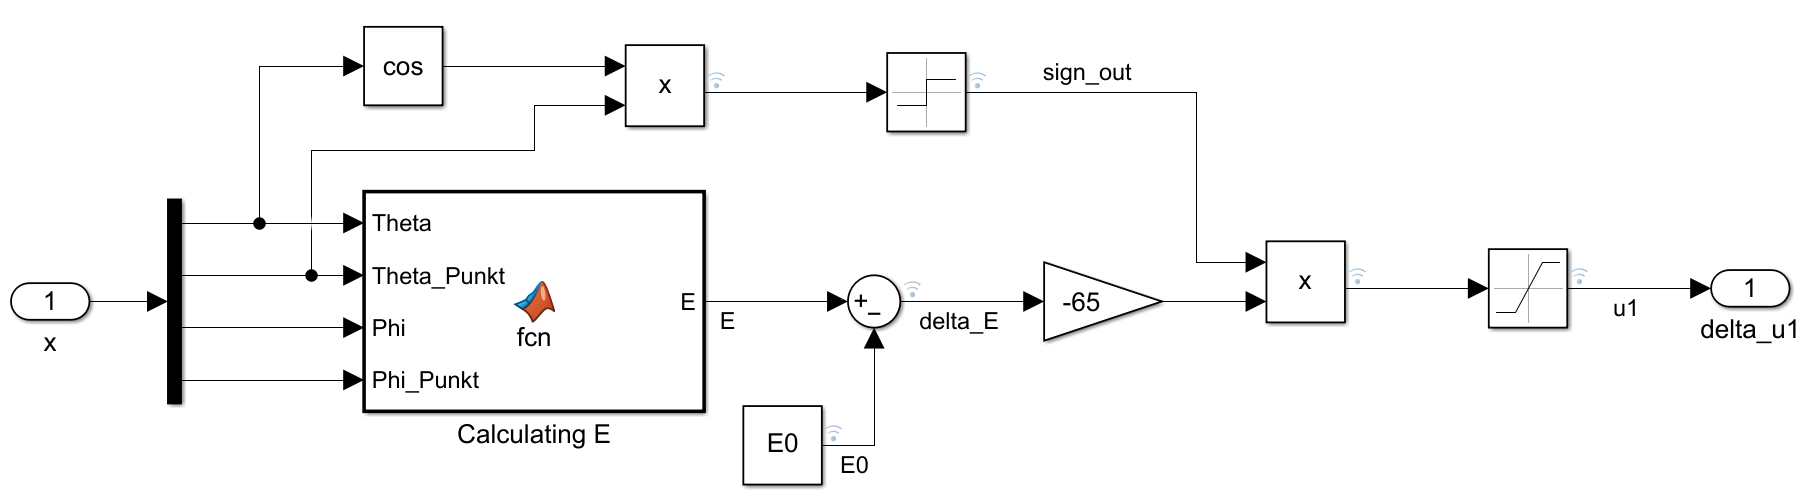
\includegraphics[width=0.95\textwidth]{Bilder/6_aufschwingen/Aufschwung-Regler_BSB.png}}
   \caption[Aufschwung-Reglerstruktur]{Aufschwung-Reglerstruktur}
   \label{fig:Bild6.1}
\end{figure}

Charmant an dieser Variante ist, dass das Energieniveau schon vor der oberen Ruhelage erreicht ist und die Energie-Zufuhr des Aktuators gestoppt wird. Die verbleibende kinetische Energie wandelt sich dann zu potentiellen Energie; während das Pendel mit dem restlichen Schwung in die obere Ruhelage läuft. Dadurch kommt das Pendel sehr ruhig in der oberen Ruhelage an und es wird ein Überschwingen vermieden.
Zur Implementierung wurden die in \autoref{sec:Modellierung} aufgestellten Energie-Gleichungen nach Lagrange genutzt – wobei die kinetische Energie des Rades in der Summe nicht berücksichtigt wird, da das den Aktuator und die Regelgröße darstellt.

\begin{equation} \label{eq:Gleichung6.2}
    E = E_{\mathrm{kin,trans}} + E_{\mathrm{pot}}
\end{equation}
\newline

Mit dieser Regelung war ein nahezu perfektes Aufschwingen möglich, bei dem der Regler nach dem Umschalten in den meisten Fällen nur noch im Bereich von ~5V gegensteuern musste, um das Pendel auf der oberen Ruheposition zu halten.

\begin{figure}[H]
   \centering
   \fbox{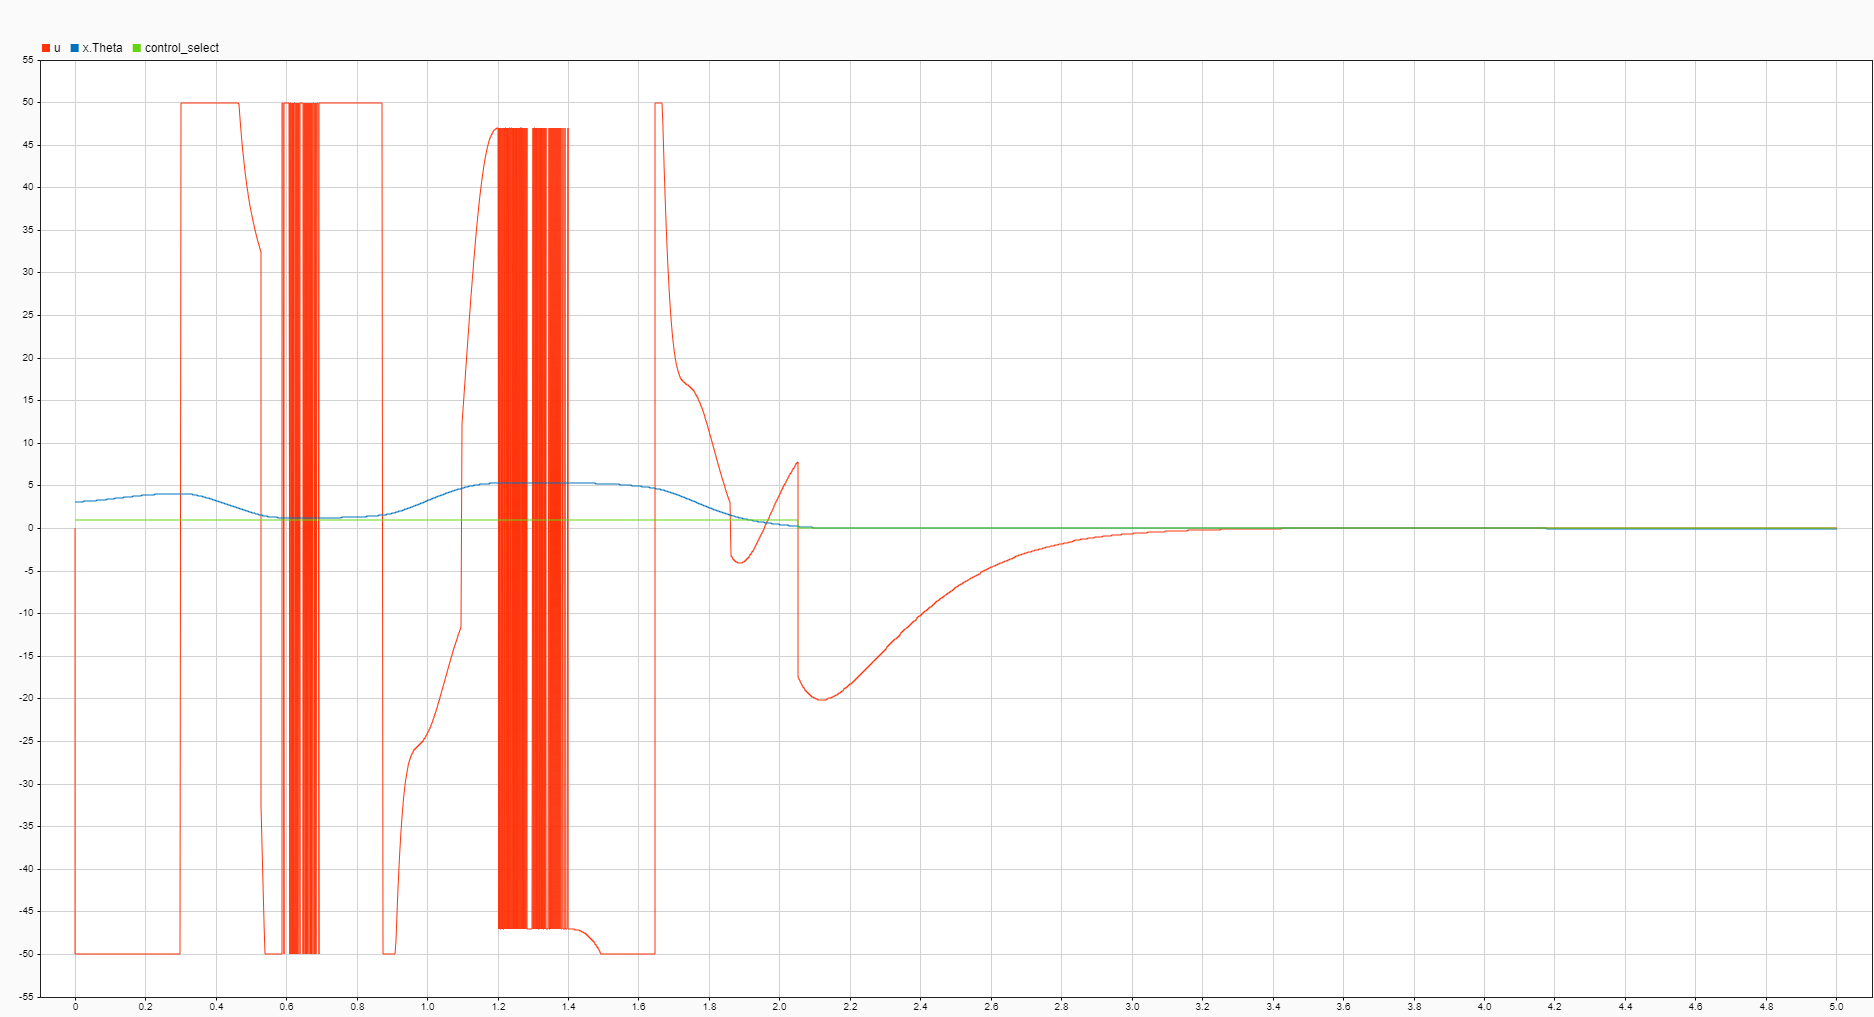
\includegraphics[width=0.95\textwidth]{Bilder/6_aufschwingen/Aufschwung-Regler.png}}
   \caption[Aufschwung-Regelung]{Aufschwung-Regelung}
   \label{fig:Bild6.2}
\end{figure}

Da in diesem Projekt aber nicht alle Zustandsvariablen gemessen werden können und stattdessen mittels einem Beobachter rekonstruiert werden sollen [vgl.: \autoref{sec:beobachter}] und dieser Beobachter nur in der Nähe des Lineariesierungs-Punktes fehlerarm arbeitet, ist die oben beschriebene Aufschwung-Regelung nicht mit dem Beobachter zu verwenden.
Daher ist in diesem Projekt ein zweiter Ansatz implementiert, welcher lediglich die aktuelle Winkelposition auswertet und wenn der aktuell gemessene Winkel kleiner als der in dem letzten Schleifen-Durchlauf ist, die Richtung des Schwungrades ändert. Schwingt das Pendel nun in einen Bereich von $\pm 14^\circ$ wird auf den Regler umgeschaltet.

\begin{figure}[H]
   \centering
   \begin{minipage}[t]{0.60\linewidth}
        \fbox{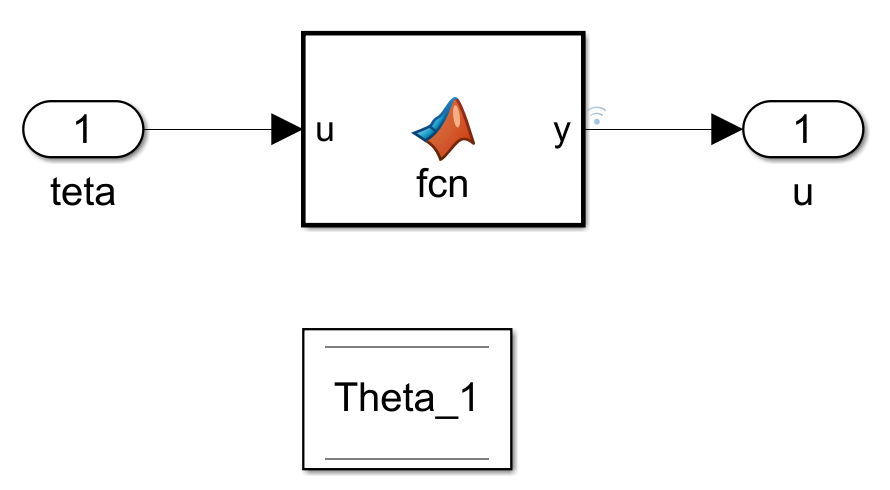
\includegraphics[width=0.95\textwidth]{Bilder/6_aufschwingen/Aufschwungsteuerung_BSB.png}}
   \end{minipage}
   \hfill
   \begin{minipage}[t]{0.3\linewidth}
        \fbox{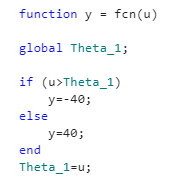
\includegraphics[width=0.95\textwidth]{Bilder/6_aufschwingen/Aufschwungsteuerung_Code.png}}
   \end{minipage}
   \caption[Aufschwung-Steuerungsstruktur]{Aufschwung-Steuerungsstruktur}
   \label{fig:Bild6.3}
\end{figure}

\begin{figure}[H]
   \centering
   \fbox{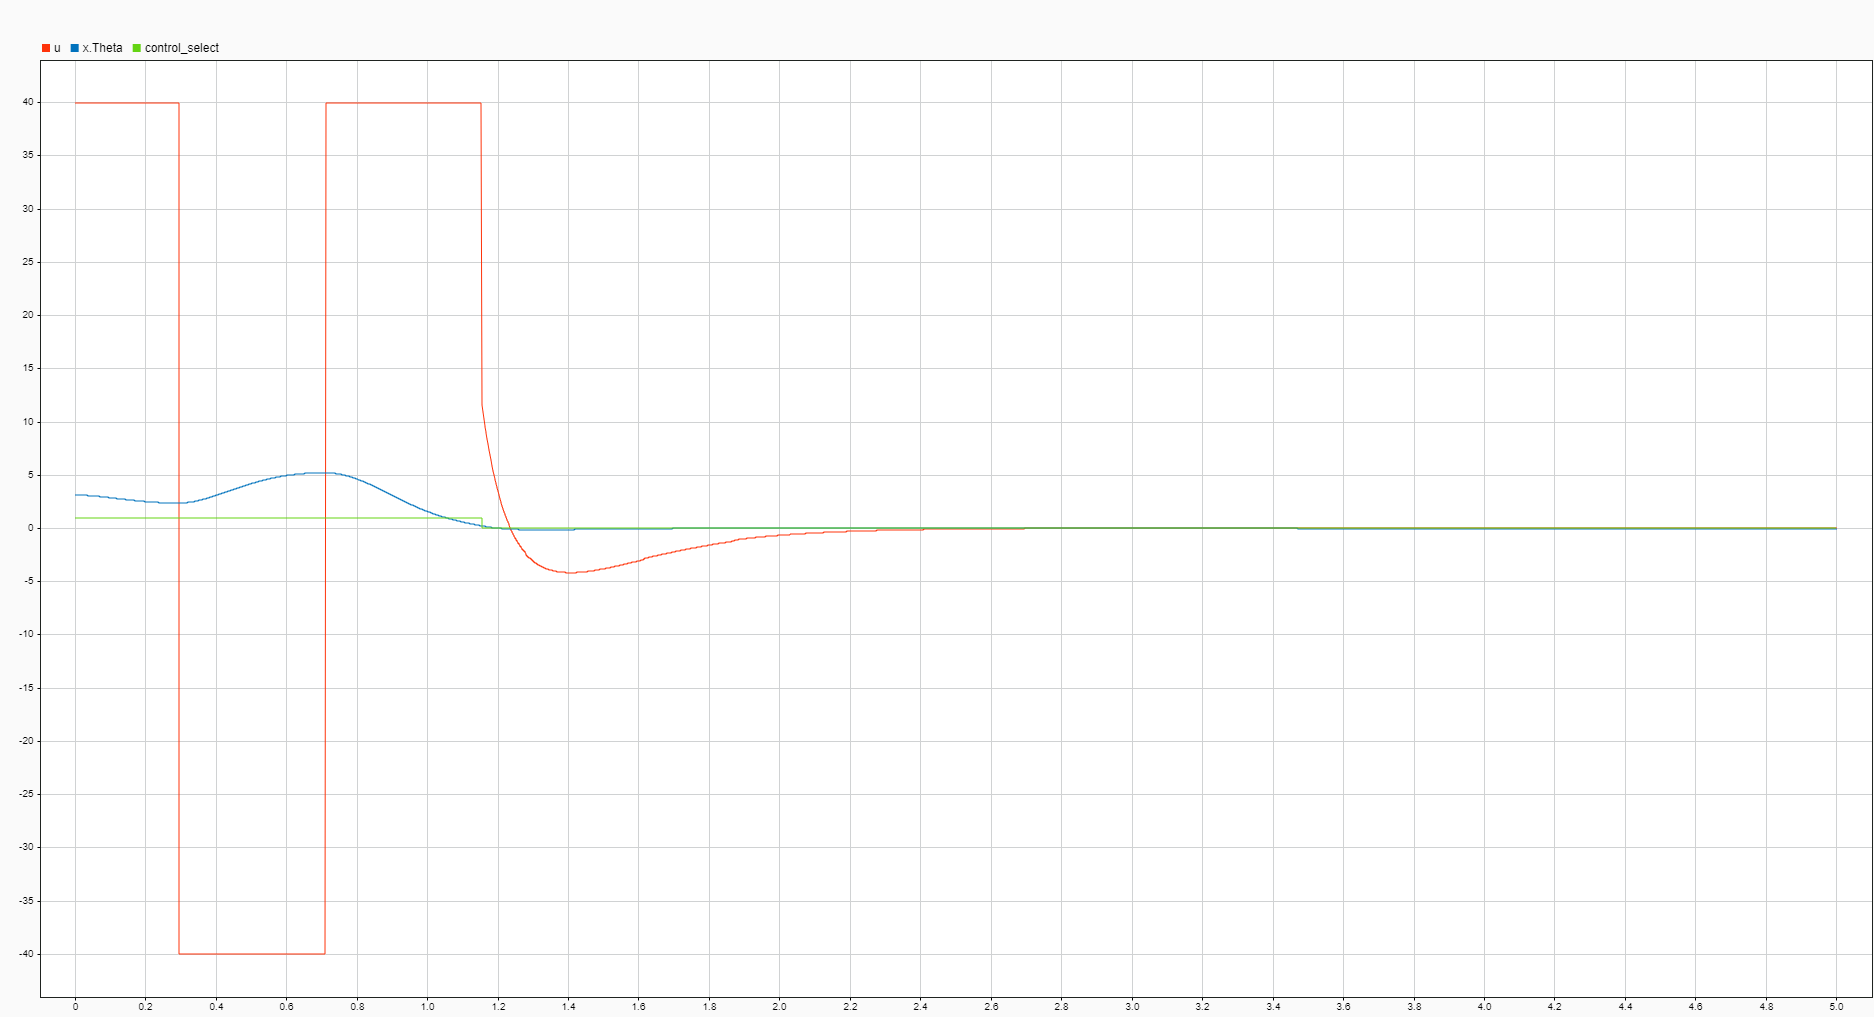
\includegraphics[width=0.95\textwidth]{Bilder/6_aufschwingen/Aufschwung-Steuerung.png}}
   \caption[Aufschwung-Steuerung]{Aufschwung-Steuerung}
   \label{fig:Bild6.4}
\end{figure}

Bei beiden Implementierungen werden die Winkel so angepasst, dass sie nur in einem Bereich von $0$ bis $2\pi$ für die Aufschwung-Steuerung respektive $-\pi$ bis $+\pi$ für den Regler liegen. Für die Aufschwung-Steuerung liegt die Unstetigkeits-Stelle in der oberen Ruhelage und für den Regler in der unteren Ruhelage. Durch die Umschaltung zwischen den beiden Regelungen erreichen die Regler niemals die Unstetigkeit während sie aktiv sind.

\begin{figure}[H]
   \centering
   \fbox{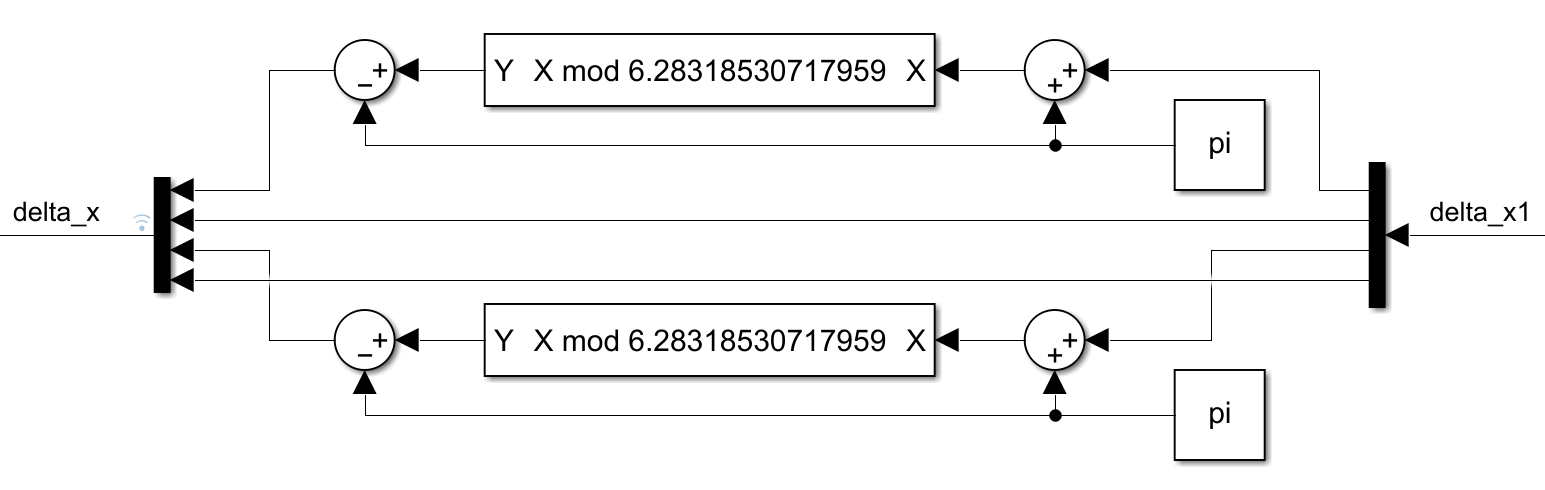
\includegraphics[width=0.95\textwidth]{Bilder/6_aufschwingen/Signal-Conditioning_for_x_BSB.png}}
   \caption[Signal-Anpassung für den Regler]{Signal-Anpassung für den Regler}
   \label{fig:Bild6.5}
\end{figure}

\begin{figure}[H]
   \centering
   \fbox{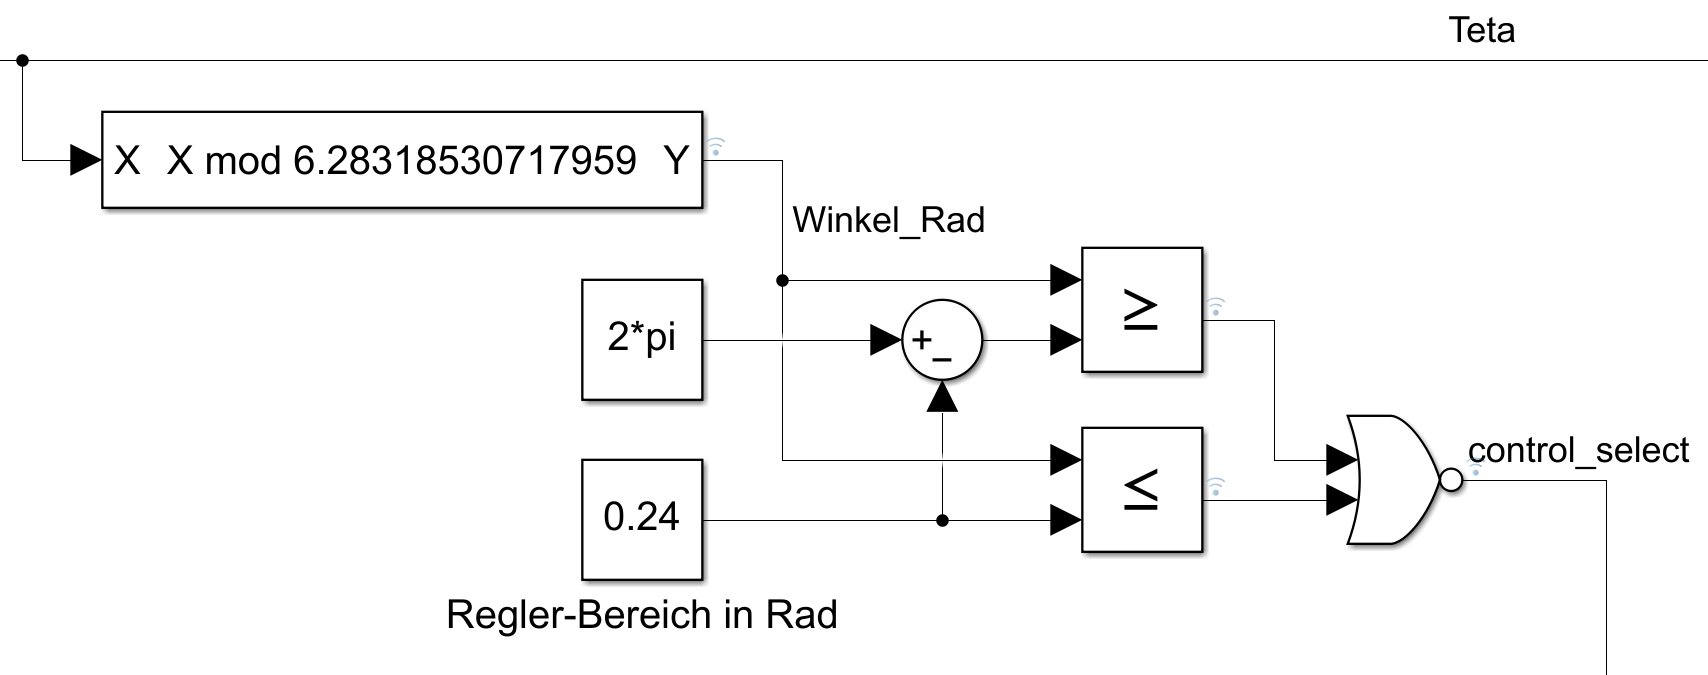
\includegraphics[width=0.95\textwidth]{Bilder/6_aufschwingen/Umschalt-Steuerung_BSB.png}}
   \caption[Umschalt-Steuerung]{Umschalt-Steuerung}
   \label{fig:Bild6.6}
\end{figure}

Es zeigte sich bei den Simulationen, dass eine maximale Motor-Spannung von 20V nicht ausreicht, um einen ausreichenden Drehmoment zu erzeugen, welcher das Pendel aufschwingen kann. Es werden bei diesem Modell mit diesem Motor mindestens 40V benötigt um das Pendel aus der unteren in die obere Ruhelage zu bewegen.
